%% !TEX root = ../Thesis.tex
%% !TEX output_directory
\documentclass[11pt,a4paper,english,greek,twoside]{../Thesis}
\usepackage{mathtools}  
\mathtoolsset{showonlyrefs}  
\begin{document}
%\everymath{\displaystyle}
\chapter{Θεωρητικό υπόβαθρο}\label{chap:Background}
\par Σε αυτό το κεφάλαιο θα παρουσιαστούν όλες οι υπολογιστικές μέθοδοι που χρησιμοποιήθηκαν σε αυτήν την διπλωματική εργασία, και που αφορούν την προ-επεξεργασία των εγκεφαλικών σημάτων, την εξαγωγή κατάλληλων-αντιπροσωπευτικών χαρακτηριστικών από τα σήματα, τα οποία θα χρησιμοποιηθούν ως είσοδος στους αλγορίθμους απόφασης και μηχανικής μάθησης. Σε αυτό το επίπεδο θα γίνει μόνο μια αναφορά στα γενικά χαρακτηριστικά της κάθε μεθόδου, οπότε είναι πιθανό να μην γίνει άμεσα αντιληπτός ο συγκεκριμένος τρόπος με τον οποίον θα εφαρμοστεί η κάθε μέθοδος στο παρών πρόβλημα. Αυτού του είδους η ανάλυση θα γίνει στις υποενότητες \ref{subsec:preprocessing} και \ref{subsec:featureExtract}
\section{Αποθορυβοποίηση - Φιλτράρισμα}
\subsection{Είδη Φίλτρων}
Γενικά η λειτουργία ενός φίλτρου μπορεί να χαρακτηριστεί από τη χαρακτηριστική του απόκριση στο πεδίο του χρόνου. Πιο συγκεκριμένα, οι πιο συχνά χρησιμοποιούμενες κατηγορίες αφορούν φίλτρα τα οποία επιτρέπουν την διέλευση συχνοτήτων από ένα κατώφλι και άνω, όπου ονομάζονται υψιπερατά, ενώ από ένα κατώφλι και κάτω, βαθυπερατά. Τέλος υπάρχουν και αυτά που είτε επιτρέπουν την διέλευση μεταξύ δύο προκαθορισμένων συχνοτήτων (ζωνοπερατά), είτε την εμποδίζουν (φραγμού-ζώνης).
\begin{figure}[H]
    \centering     %%% not \center
    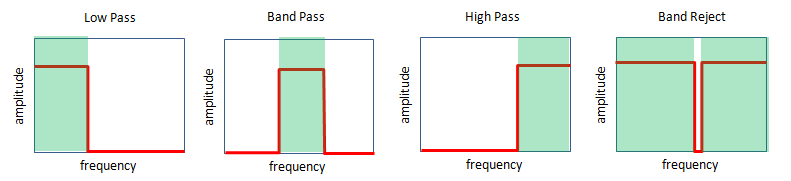
\includegraphics[scale=0.7]{{ImagesSSVEP/filter_types}.png}
    \caption{Τα τέσσερα βασικά είδη φίλτρων με βάση τις ζώνες συχνοτήτων που επιτρέπουν-απορρίπτουν. Αξίζει να σημειωθεί πως οι υποφαινόμενες αποκρίσεις στο πεδίο της συχνότητας, αναφέρονται σε ιδανικά φίλτρα (brick-wall filters), και πως στα πραγματικά, οι ζώνες αποκοπής δεν ορίζονται ποτέ από κάθετες γραμμές.}
    \label{fig:filter_types}
\end{figure}
\par Ένα άλλο κριτήριο με βάση το οποίο διαχωρίζονται τα φίλτρα είναι ο τρόπος με τον οποίο κάθε στιγμή χειρίζονται τις προηγούμενες εισόδους και εξόδους του συστήματος. Τα φίλτρα των οποίων η έξοδος εξαρτάται μόνο από τις προηγούμενες εισόδους ονομάζονται Φίλτρα Πεπερασμένης Κρουστικής Απόκρισης (Finite Impulse Response - FIR), ενώ αυτά που λαμβάνουν υπόψιν τους τόσο τις προηγούμενες εισόδους, αλλά και τις προηγούμενες εξόδους ονομάζονται Φίλτρα Άπειρης Κρουστικής Απόκρισης (Infinite Impulse Response - IIR). Το γεγονός πως τα IIR χρησιμοποιούν ένα είδος ανάδρασης (εξάρτηση από προηγούμενες εισόδους) είναι δυνατόν να τα καταστήσει ασταθή, πράγμα το οποίο δεν συμβαίνει με τα FIR, αν όμως χρησιμοποιηθεί με σωστό τρόπο, τότε, δεδομένων κάποιων συγκεκριμένων προδιαγραφών για ένα φίλτρο, μια IIR υλοποίηση θα ικανοποιήσει τις προδιαγραφές κάνοντας χρήση φίλτρου τάξης πολύ χαμηλότερης από το αντίστοιχο FIR, το οποίο μεταφράζεται σε λιγότερες πράξεις, άρα και σε λιγότερο υπολογιστικό χρόνο. 

\par Ένα από τα πιο κλασσικά IIR φίλτρα σχεδιάστηκε το 1930 απο το βρετανό μηχανικό και φυσικό Stephen Butterworth \cite{}. Βασικός στόχος του φίλτρου αυτού ήταν η επίτευξη σταθερής απόκρισης στη περιοχή διέλευσης συχνοτήτων, σε αντίθεση με τα μέχρι τότε φίλτρα τα οποία εμφάνιζαν διακυμάνσεις στην απόκρισή τους (ripple). Το τίμημα όμως για αυτήν την συμπεριφορά, είναι πως υπάρχει σχετικά μεγάλη απόκλιση στην περιοχή της συχνότητας αποκοπής, συγκριτικά με την απόκριση του αντίστοιχου ιδανικού φίλτρου.
\begin{figure}[H]
    \centering     %%% not \center
    \noindent\makebox[\textwidth]{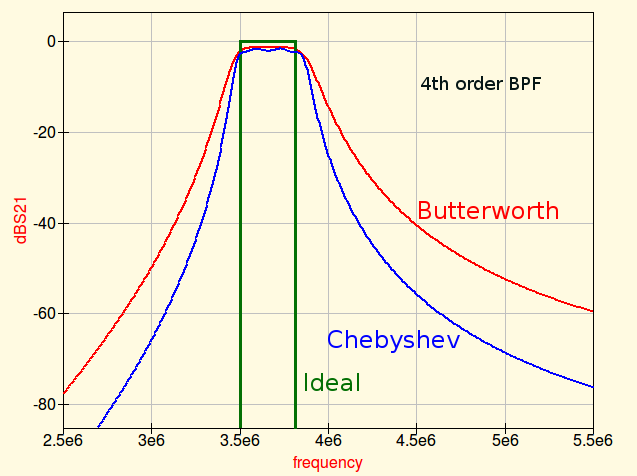
\includegraphics[scale=0.6]{{ImagesSSVEP/butter_cheby}.png}}
    \caption{Οι τρείς διαφορετικές αποκρίσεις για δύο διαφορετικά φίλτρα 3ης τάξης και του αντίστοιχου ιδανικού. Φαίνεται ξεκάθαρα η διακύμανση (ripple) στην ζώνη διέλευσης για ένα φίλτρο τύπου Chebyshev, η οποία δεν υπάρχει στο Butterwoth, καθώς και η μεγάλη απόκλιση του Butterworth σε σχέση με το ιδανικό, όσον αφορά τις δύο ζώνες αποκοπής. }
    \label{fig:butter_cheby}
\end{figure}
% add butte2

\section{Εξαγωγή χαρακτηριστικών - Μηχανική Μάθηση}

\subsection{Φασματική Ανάλυση Ισχύος - Power Spectral Density (PSD)}

\par Η φασματική ανάλυση μελετάει το τρόπο με τον οποίον η συνολική ενέργεια ενός σήματος κατανέμεται σε κάθε για από τις συχνότητες που το αποτελούν. Μια από τις πρώτες και πιο απλές μεθόδους προσέγγισης του PSD είναι το περιοδόγραμμα, το οποίο μπορεί για ένα συνεχές σήμα $x(t)$ ορίζεται ως:
\begin{align}
P_x(f)&=\frac{1}{T}\left|\int_0^Tx(t)e^{-j2\pi ft}dt\right|^2
\label{eqPSD1}
\end{align}
\par Δειγματοληπτώντας το σήμα $x(t)$ σε $N$ σημεία, ανά $Ts$, τότε προκύπτει το σήμα διακριτού χρόνου $x[n] = x(t)\sum_{n\in\mathbb{Z}} \delta(t-nT_s)$, και επομένως η διακριτή προσέγγιση της εξίσωσης \eqref{eqPSD1} είναι η εξής:
\begin{align}
    \begin{split}
        P_x(f)\approx &\frac{1}{NT_s}\left|\sum_{n=0}^{N-1}x[n]e^{-j2\pi fnT_s}\cdot T_s\right|^2 \\[2ex]
        =&\frac{T_s}{N}\left|\sum_{n=0}^{N-1}x[n]e^{-j2\pi fnT_s}\right|^2
        \label{eqPSD2}
    \end{split}
\end{align}
\par Υπολογίζοντας τώρα την \eqref{eqPSD2}, σε διακριτές ισαπέχουσες συχνότητες $f_k=kf_s/K$, $k=0,1,\ldots K-1$, όπου $f_s=1/T_s$, και $K\ge N$, τότε προκύπτει:
\begin{align}
    P_x\left(\frac{kf_s}{K}\right)\approx &\frac{T_s}{N}\left|\sum_{n=0}^{N-1}x[n]e^{-j2\pi kn/K}\right|^2=\frac{T_s}{N}\left|X[k]\right|^2
    \label{eqPSD3}
\end{align}
\par όπου $X[k]$ είναι ο διάστασης $K$ διακριτός μετασχηματισμός Fourier (DFT) του σήματος $x[n]$. Στην περίπτωση όπου $K>N$, τότε προστίθονται $K-N$ μηδενικά στο $x[n]$ (zero-padding). Στην περίπτωση όπου o DFT υπολογιστεί μόνο από την μια πλευρά του (άθροισμα σε $N/2$ στοιχεία αντί για $N$, τότε ο συντελεστής $T_s/N$ θα πρέπει να διπλασιαστεί. 
\par Τέλος, πολύ συχνά εφαρμόζεται ένα παράθυρο $w[n]$ στο σήμα $x[n]$, πριν υπολογιστεί ο PSD, και σε αυτή την περίπτωση ο όρος $N$ στον συντελεστή κανονικοποίησης αλλάζει, και έχουμε:
\begin{align}
    P_x\left(\frac{kf_s}{K}\right)\approx &\frac{T_s}{W}\left|X[k]\right|^2 , \ \text{με} \ \ W=\sum_{i=1}^{N} w_{i}^{2}
    \label{eqPSD4}
\end{align}
\par Παρατηρούμε πως στην περίπτωση τετραγωνικού παραθύρου, τότε $W=N$.
\par Η πληροφορίες που μας παρέχει η φασματική ανάλυση ενός σήματος είναι καθοριστικής σημασίας. Η γνώση των επικρατέστερων συχνοτήτων που αποτελούν το σήμα, μας δίνει την δυνατότητα να κατασκευάσουμε αρκετά αντιπροσωπευτικό σύνολο χαρακτηριστικών για αυτό, και παρότι οι μέθοδοι που βασίζονται στον μετασχηματισμό Fourier είναι επιρρεπής στην λάθος ανίχνευση συχνοτήτων, παρουσία θορύβου στο σήμα, θα δούμε πως σε συνδυασμό με άλλες μεθόδους και τεχνικές, δίνουν πολύ καλά αποτελέσματα. 

\subsection{Ανάλυση Κύριων Συνιστωσών - Principal Component Analysis (PCA)}
\par Η Ανάλυση Κυρίων Συνιστωσών είναι μια στατιστική μέθοδος, που στο τομέα της μηχανικής μάθησης χρησιμοποιείται πολύ συχνά για την ελάττωση των χαρακτηριστικών (features) των δειγμάτων ενός συνόλου, επιλέγοντας μόνο εκείνα τα χαρακτηριστικά τα οποία συνεισφέρουν στην διατήρηση του μεγαλύτερου ποσοστού της μεταβλητότητας (variance) του συνόλου. Μια γεωμετρική ερμηνεία της παραπάνω διαδικασίας, είναι η προσπάθεια εύρεσης των κατευθύνσεων - αξόνων μέγιστης μεταβλητότητας των δεδομένων, και η προβολή τους σε κάποιους από αυτούς τους άξονες.

\begin{figure}[H]
    \centering     %%% not \center
    \subfigure[]{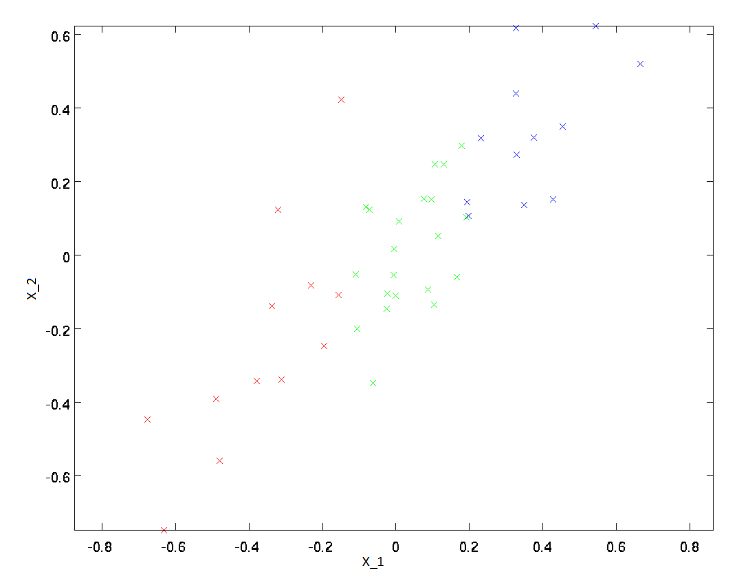
\includegraphics[width=60mm,height=50mm]{{{ImagesSSVEP/PCA1}.PNG}}}
    \subfigure[]{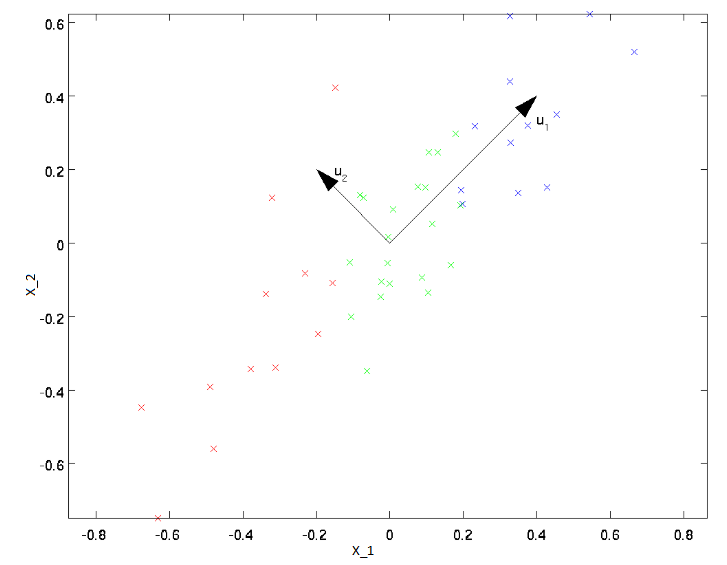
\includegraphics[width=60mm,height=50mm]{{{ImagesSSVEP/PCA2}.PNG}}}
    \subfigure[]{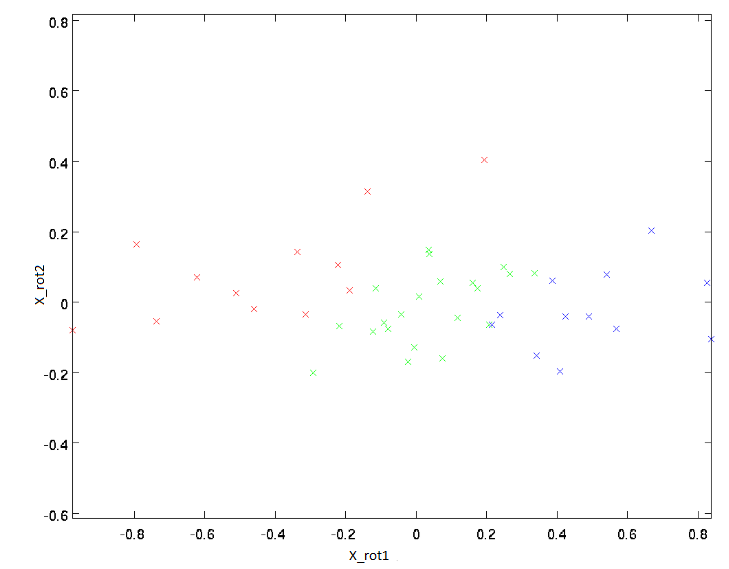
\includegraphics[width=60mm,height=50mm]{{{ImagesSSVEP/PCA3}.PNG}}}
    \subfigure[]{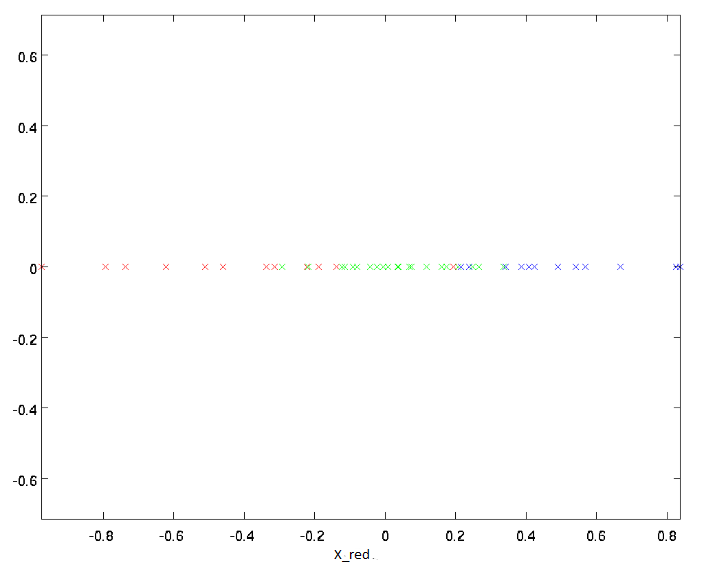
\includegraphics[width=60mm,height=50mm]{{{ImagesSSVEP/PCA4}.PNG}}}
    \caption{Γεωμετρική ερμηνεία της PCA. a) Η αναπαράσταση ενός συνόλου δισδιάστατων δειγμάτων στο καρτεσιανό επίπεδο. b) Η PCA βρίσκει τις κατευθύνσεις μέγιστης μεταβλητότητας-διασποράς. Με το μάτι εύκολα καταλήγουμε πως η μέγιστη κατεύθυνση είναι η $u_1$, ενώ η $u_2$ είναι η αμέσως επόμενη ορθογώνια. c) Η περιστροφή των δεδομένων ως προς την νέα ορθογώνια βάση $(u_1,u_2)$. d) Ελάττωση της διάσταση των δειγμάτων, προβάλλοντας τα στον άξονα μέγιστης διακύμανσης.}
    \label{fig:pca}
\end{figure}
 

\par Η χρησιμότητα της μεθόδου αυτής είναι εμφανής όταν έχουμε πολυδιάστατα δείγματα, όπως για παράδειγμα εικόνες  μεγέθους 16x16, δηλαδή δυανύσματα χαρακτηριστικών που ανήκουν στο $R^{256}$. Η χρήση όλων αυτών των χαρακτηριστικών σε έναν ακριβά υπολογιστικό αλγόριθμο μηχανικής μάθησης, όπως ο k-NN, θα επιβάρυνε σημαντικά την διαδικασία απόφασης, τόσο υπολογιστικά όσο και χρονικά. Με την χρήση της PCA όμως, είναι δυνατό να επιλεχθεί ένας αριθμός χαρακτηριστικών (π.χ 50-60), τα οποία να διατηρούν την πιο σημαντική στατιστική πληροφορία του συνόλου των εικόνων, με αποτέλεσμα να ελαττώνονται σημαντικά οι πόροι που χρείαζονται για την ταξινόμηση τους, χωρίς την εισαγωγή σημαντικού σφάλματος ταξινόμησης. Τέλος, ένα επιπλέον πλεονέκτημα, είναι πως σε πολλές περιπτώσεις, η PCA, βοηθάει στην αποφυγή του overfitting.

\par Όσον αφορά τον τρόπο υπολογισμού των κύριων συνιστωσών, θα δώσουμε ένα παράδειγμα (εικόνα \ref{fig:pca}), για ένα σύνολο δειγμάτων $X$ όπου το καθένα έχει δύο χαρακτηριστικά, δηλαδή $X_i \epsilon R^2$, όπου ο σκοπός μας είναι να του ελαττώσουμε την διάσταση κατά ένα. Αρχικά υπολογίζουμε τον πίνακα 
\begin{align}
\Sigma = \frac{1}{m}\sum_{i=1}^{i=m} X_i(X_i)^T \label{eq1}
\end{align}

\par Υποθέτοντας πως τα δεδομένα μας είναι κανονικοποιημένα έτσι ώστε $E[X_i]=0$ τότε η εξίσωση \eqref{eq1} ορίζει τον πίνακα συνδιασποράς του συνόλου $X$. Αποδεικνύεται πως η κατεύθυνση μέγιστης μεταβλητότητας $u_1$ (εικόνα \ref{fig:pca}) αντιστοιχεί στο ιδιοδιάνυσμα που προκύπτει από την μεγαλύτερη ιδιοτιμή του πίνακα $\Sigma$. Αντίστοιχα η αμέσως επόμενη κατεύθυνση μέγιστης μεταβλητότητας $u_2$, αντιστοιχεί στο ιδιοδιάνυσμα που προκύπτει από την αμέσως μικρότερη ιδιοτιμή. Γενικεύοντας τώρα την παραπάνω πρόταση, αν τα δεδομένα μας $X_i \epsilon R^n$, και θέλουμε να τα προβάλουμε σε έναν υποχώρο διάστασης $R^k$, $k<n$, τότε πρέπει να διαλέξουμε τα $u_1,...,u_k$ να είναι τα ιδιοδιανύσματα που προκύπτουν από τις $k$ μεγαλύτερες ιδιοτιμές του πίνακα $\Sigma$, ο οποίος επειδή είναι συμμετρικός, τότε τα $u_i$, μπορούν πάντα να επιλέγονται έτσι ώστε να σχηματίζουν μια νέα ορθογώνια βάση για τα δεδομένα.

\par Στην συνέχεια του παραδείγματος μας τώρα, αφού υπολογίσουμε τα δύο ιδιοδιανύσματα $u_1$ και $u_2$ τότε μπορούμε να αναπαραστήσουμε τον πίνακα δεδομένων $X$, ως προς την ορθογώνια βάση $(u_1,u_2)$
\begin{align}
X_{rot} = U^TX =\begin{bmatrix}u_1^T\\u_2^T\end{bmatrix}X= \begin{bmatrix}u_1^TX\\u_2^TX\end{bmatrix}
\label{eq2}
\end{align}
\par Χρησιμοποιήθηκε ο δείκτης rot για τα μετασχηματισμένα δεδομένα, καθώς ο πολλαπλασιασμός του $X$ με τον ορθογώνιο πίνακα $U$, υποδηλώνει την περιστροφή του $X$.
\par Προκειμένου τώρα να ελαττώσουμε την διάσταση των δεδομένων, θα κρατήσουμε μόνο το μέρος του $X_{rot}$ που προέρχεται από την κύρια συνιστώσα, δηλαδή το ιδιοδιάνυσμα $u_i$. Συνεπώς η νέα εξίσωση για την αναπαράσταση του $X$ σε μία διάσταση θα είναι:
\begin{align}
X_{red} = U_{red}^TX =\begin{bmatrix}u_1^T\end{bmatrix}X= \begin{bmatrix}u_1^TX\end{bmatrix}
\label{eq3}
\end{align}
\subsection{Ανάλυση Κανονικής Συσχέτισης - Canonical Correlation Analysis (CCA)}

\par Η CCA είναι μια στατιστική μέθοδος που αναπτύχθηκε από τον Hotelling \cite{Hotelling1936-vk} και χρησιμοποιείται για την ανάλυση δομών δεδομένων, και συγκεκριμένα για την ανίχνευση της ομοιότητας μεταξύ δύο συνόλων μεταβλητών. Αυτό επιτυγχάνεται μέσω της εύρεσης δύο νέων συνόλων μεταβλητών, όπου το καθένα είναι γραμμικός συνδυασμός ενός από τα αρχικά σύνολα, έτσι ώστε να μεγιστοποιείται ο συντελεστής συσχέτισης τους. 
\par Κάνοντας χρήση μαθηματικού φορμαλισμού, έστω δύο πολυδιάστατες και τυχαίες μεταβλητές $X$ και $Y$, και οι γραμμικοί συνδυασμοί τους $x=X^Ta$ και $y=Y^Tb$, αντίστοιχα. Για τον συντελεστή συσχέτισης μεταξύ των $x$ και $y$ έχουμε:
\begin{align}
\begin{split} %\max_{a,b}
p(x,y)&=\frac{Cov(x,y)}{\sqrt{Cov(x,x)Cov(y,y)}} \\[2ex]
&=\frac{E[(x-E[x])(y-E[y])]}{\sqrt{E[(x-E[x])^2]E[(y-E[y])^2]}} \\[2ex]
&=\frac{E[a^T(X-E[X])(Y-E[Y])^Tb]}{\sqrt{E[(a^T(X-E[X]))^2]E[((Y-E[Y])^Tb)^2]}} \\[2ex]
&=\frac{a^TCov(X,Y)b}{\sqrt{a^TCov(X,X)ab^TCov(Y,Y)b}} \\
\label{eqCCA1}
\end{split}
\end{align}

\par H CCA προσπαθεί να υπολογίσει τα $a, b$ έτσι ώστε να μεγιστοποιηθεί ο παραπάνω συντελεστής συσχέτισης, λύνοντας το ακόλουθο πρόβλημα:
\begin{align}
\max_{a,b}p(x,y)=\frac{a^TCov(X,Y)b}{\sqrt{a^TCov(X,X)ab^TCov(Y,Y)b}} \\
\label{eqCCA2}
\end{align}

\par Έστω $x=x_1,y=y_1$. Το ζεύγος των μεταβλητών $(x_1, y_1)$ ονομάζεται πρώτο ζεύγος κανονικών μεταβλητών, και ο αντίστοιχος συντελεστής $p_1$, πρώτη κανονική συσχέτιση. Όμοια ορίζουμε και όλα τα ζεύγη κανονικών μεταβλητών, $(x_1,y_1),(x_2,y_2),...,(x_k,y_k)$, τα οποία οποία αντιστοιχούν στις κανονικές συσχετίσεις $p_1,p_2,...p_k$ τέτοιες ώστε $1\leq p_1\leq p_2\leq ... \leq p_k$

\textbf{Ποια ειναι η λυση τελικα ? Ιδιοτιμες}

\textbf{Ομοιότητες CCA και PCA} 
\par Όπως είπαμε η CCA προσπαθεί να βρει την ομοιότητα μεταξύ των $Χ,Y$ υπολογίζοντας τα κανονικά ζεύγη μεταβλητών, και ορθογώνια μεταξύ τους, $(x_k,y_k)$. Το πρώτο κανονικό ζεύγος μεταβλητών $(x_1, y_1)$ αποτυπώνει το μεγαλύτερο μέρος αυτής της ομοιότητας, αλλά όχι ολόκληρο. Όσο περισσότερα ζεύγη συμπεριλαμβάνονται, τόσο μεγαλύτερο ποσοστό αποτυπώνεται. Από αυτή την περιγραφή προκύπτει η αναλογία με την μέθοδο PCA. Στην PCA, προσπαθούμε να υπολογίσουμε ορθογώνιες μεταξύ τους κύριες συνιστώσες-κατευθύνσεις μέσα στον πολυδιάστατο χώρο μιας μόνο μεταβλητής. Η πρώτη κύρια συνιστώσα αποτυπώνει το μεγαλύτερο ποσοστό μεταβλητότητας-διασποράς, το οποίο αυξάνεται, με την αύξηση των εναπομεινάντων κυρίων συνιστωσών. Άρα συνολικά μπορούμε να πούμε πως με την CCA προσπαθούμε να βρούμε την ομοιότητα μεταξύ δύο διαφορετικών πολυδιάστατων μεταβλητών, ενω με την PCA, την διαφορετικότητα μέσα στην ίδια μεταβλητή.

\subsection{κ-Κοντινότεροι Γείτονες - k-Nearest Neighbors (k-NN)}
\par Ο k-NN, είναι ένας από τους απλούστερους αλγορίθμους επιβλεπόμενης μηχανικής μάθησης, και βασίζεται στην χρήση μέτρων απόστασης μεταξύ του δείγματος προς ταξινόμηση και των δειγμάτων που αποτελούν το σύνολο εκπαίδευσης. Ο k-NN, σε αντίθεση με άλλους αλγορίθμους μηχανικής μάθησης, δεν βασίζεται σε κάποιο στατιστικό μοντέλο το οποίο να υποθέτει κάποια κατανομή στην οποία υπακούν τα χαρακτηριστικά του δείγματος. Αντιθέτως, το μοντέλο είναι τα ίδια τα δείγματα αποθηκευμένα μαζί με τις ετικέτες τους για την κλάση στην οποία ανήκουν.
\par Έστω τα δείγματα $X_1,X_2,...,X_m$, όπου $n$, ο αριθμός των χαρακτηριστικών του καθενός. Ο k-NN υποθέτει πως τα $X_i$ είναι σημεία του n-διάστατου χώρου, δηλαδή $X_i\epsilon R^n$. Το σύνολο εκπαίδευσης θα αποτελείται από δείγματα της μορφής ${X-i,c_i}$, όπου το $c_i$ είναι η ετικέτα (label) που δηλώνει την κλάση στην οποία ανήκει το κάθε δείγμα εκπαίδευσης. Στο επόμενο στάδιο, ένα νέο δείγμα $Y_i \epsilon R^n$, του οποίου δεν γνωριίζουμε την ετικέτα (unlabeled), ταξινομείται με τον εξής τρόπο. Πρώτα υπολογίζεται η απόσταση του ως προς καθένα από τα δείγματα εκπαίδευσης. Συνήθως χρησιμοποιείται η ευκλείδεια απόσταση, αλλά συχνά γίνεται χρήση και άλλων όπως Mahalanobis, Manhattan, cosine similarity, dynamic time wrapping κ.α. Στην συνέχεια επιλέγονται οι k κοντινότεροι γείτονες, δηλαδή τα δείγματα εκπαίδευσης με την μικρότερη απόσταση από το νέο δείγμα, και στο οποίο αναθέτουμε την ετικέτα της πλειοψηφίας των k γειτόνων του.
\begin{figure}[H]
    \centering     %%% not \center
    \noindent\makebox[\textwidth]{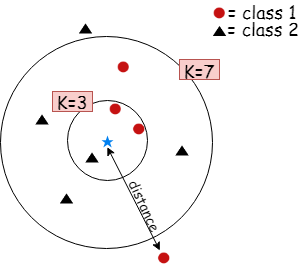
\includegraphics[scale=0.6]{{ImagesSSVEP/kNN_diagram}.png}}
    \caption{Γραφική αναπαράσταση του αλγορίθμου k-NN. Το μπλε αστέρι δηλώνει το δείγμα προς ταξινόμηση. Στην περίπτωση όπου K=3, τότε το δείγμα ταξινομείται στην κλάση 1, καθώς έχουμε δύο κύκλους και ένα τρίγωνο. Στην περίπτωση όπου K=7, τότε ταξινομείται στην κλάση 2, καθώς αυτή είναι η κλάση της πλειοψηφίας των γειτόνων.}
    \label{fig:kNN}
\end{figure}
\subsection{Πολυμεταβλητή Γραμμική Παλινδρόμηση - Multivariate Linear Regression (MLR)}
\cite{Wang2015-oa} Wang2015-oa
\par Η MLR (πολυμεταβλητή γραμμική παλινδρόμηση), είναι μια πολύ καλά μελετημένη μέθοδος γραμμικής παλινδρόμησης. Η παλινδρόμηση είναι ο τομέας της στατιστικής που μελετάει την ύπαρξη σχέσης μεταξύ ανεξάρτητων (ερμηνευτικών) και εξαρτημένων (ερμηνευομένων) μεταβλητών. Ανάλογα με την ποσότητα των ανεξάρτητων και εξαρτημένων μεταβλητών ονομάζουμε και διαφορετικά το μοντέλο της παλινδρόμησης. H MLR αναφέρεται στην περίπτωση που έχουμε παραπάνω από μία ανεξάρτητες και επίσης παραπάνω από μία εξαρτημένες μεταβλητές, και δεν πρέπει να συγχέεται με την πολλαπλή γραμμική παλινδρόμηση, καθώς αυτή αναφέρεται στην περίπτωση πολλαπλών μεν ανεξάρτητων μεταβλητών, αλλά μόνο μίας εξαρτημένης.

\par Η MLR μπορεί να χρησιμοποιηθεί και για προβήματα ταξινόμησης, αν ώς ανεξάρτητη μεταβλητή θέσουμε τα δεδομένα εκπαίδευσης, και ως εξαρτημένη, έναν πίνακα ετικετών (label matrix) ο οποίος περιέχει την πληροφορία για την κλάση κάθε δείγματος εκπαίδευσης. Αρχικά ας θεωρήσουμε τα δεδομένα εκπαίδευσης (ανεξάρτητες μεταβλητές) 
\begin{align}
X=[x_1,x_2...,x_N] \epsilon \mathbb{R}^{PxN}
\end{align}
, όπου $N$ ο αριθμός των δειγμάτων και $P$ ο αριθμός των χαρακτηριστικών κάθε δείγματος. Για ένα πρόβλημα ταξινόμησης $M$ κλάσεων, ο πίνακας με τις ετικέτες κατασκευάζεται θέτοντας ως στήλες τις ετικέτες $y_i$ κάθε δείγματος $x_i$, που ανήκει στην κλάση $m$, τότε 
\begin{align}
    y_i=[y_i^1,...,y_i^M]^T
    , \  
    y_i=
    \begin{cases}
      0, & \text{if}\ j\neq m \\
      1, & \text{if}\ j=m
    \end{cases}
    \label{eqMLR1}
  \end{align}
\par 
Συνεπώς, 
\begin{align}
Y=[y_1,y_2,...,y_N] \epsilon \mathbb{R}^{MxN}
\end{align}
\par Για το πρόβλημα της ταξινόμησης λοιπόν, ο MLR προσπαθεί να υπολογίσει έναν πίνακα $W \epsilon \mathbb{R}^{MxN}$ , ο οποίος πολλαπλασιαζόμενος με καθένα δείγμα $x_i$, θα δίνει αποτέλεσμα $\overline{y_i}$ το οποίο θα προσεγγίζει το $y_i$ με το μικρότερο δυνατό σφάλμα. Δηλαδή
\begin{align}
\begin{split}
&\min \frac{1}{2}\sum_{i=1}^{N}\Vert y_i-\overline{y_i}\Vert_2^2 \\[2ex]
=&\frac{1}{2}\sum_{i=1}^{N}\Vert y_i-(W^Tx_i+b)\Vert_2^2 \\[2ex]
\label{eqMLR2}
\end{split}
\end{align}
\par Όπου $b$ ο σταθερός όρος (intercept) που μπορεί να απαλειφθεί, αν κεντράριστούν τα $X$ και $Y$ γύρω από το 0. Συνεπώς για το $W$ θα έχουμε την απλουστευμένη σχέση
\begin{align}
\begin{split}
W=&\argmin_W \frac{1}{2}\sum_{i=1}^{N}\Vert y_i-\overline{y_i}\Vert_2^2 \\[2ex]
=&\argmin_W\frac{1}{2}\sum_{i=1}^{N}\Vert y_i-W^Tx_i\Vert_2^2 \\[2ex]
=&\argmin_W\frac{1}{2}\Vert Y-W^TX\Vert_F^2
\label{eqMLR3}
\end{split}
\end{align}

\par H λύση δίνεται από την σχέση
\begin{align}
W=(XX^T)^{\dagger} XY^T
\label{eqMLR4}
\end{align}
\par Όπου με $\Vert .\Vert_F$ συμβολίζεται η νόρμα Frobenius, και με $(.)^{\dagger}$ ο Moore-Penrose ψευδοαντίστροφος πίνακας. Η προσέγγιση του label matrix $Υ$, είναι η $\overline{Y}=W^TX=[]$. Ο πίνακας αυτός δεν θα περιέχει 1 και 0 όπως ο $Y$, αλλά συνεχής τιμές, συνεπώς δεν θα μπορεί να προκύψει άμεσα η απάντηση για την κλάση στην οποία ανήκει κάθε δείγμα. Επομένως χρειάζεται να γίνουν διαδικασίες που θα μετατρέψουν τον $\overline{Y}$ σε δυαδικό. Οι διαδικασίες αυτές μπορεί να κυμαίνονται από μια απλή κατωφλιοποίηση  ή εφαρμογή συνάρτησης μεγίστου, μέχρι την χρήση των διανυσμάτων $\overline{y_i}$ ως νέων αντιπροσωπευτικών χαρακτηριστικών (features) κάθε δείγματος, ώστε να χρησιμοποιηθούν ως είσοδο σε αλγορίθμους μηχανικής μάθησης.
\par Κοιτώντας την MLR από αυτή την οπτική γωνία, είναι λογικό να πούμε πως μπορεί να χρησιμοποιηθεί και ως αλγόριθμος-μετασχηματισμός για την εύρεση κατάλληλων χαρακτηριστικών.

\end{document}
